\section{Multi-Agent Source Localization}
\label{sec:03_multiAgentLoca}

The final whistle sound source localization is realized by collecting the
all \ac{WSDE} results of all active robots and combining the directions
into one xy-position outcome.
Two separate implementation details are covered in the following.
First, the actual localization algorithm that concludes the source localization
task is set in focus.
How the process of the multi-agent decision proceeds including the communication
is dealt within \cref{subsec:03_teamCommunication}.

Exemplary, two robots at position $\vec{p_1}$ and $\vec{p_2}$ with their \ac{WSDE} results
are illustrated in \cref{fig:03_rays}.
Every robot's result is represented as \textit{ray} which consists of the robot position
$\vec{p_j}$ and the \ac{WSDE} angle $\Phi_j$, both in field coordinates.
The \ac{WSDE} angle $\gamma_j$ is defined relative to the robot and the robot's orientation $\theta$
is known by its team message information.
Thus, the absolute angle is
\bal
\Phi_j &= \theta_j + \gamma_j\\
\intertext{from which the whistle source direction ray can be described as}
\vec{r_j} &= \vec{p_j} + \vec{d_j} % = \begin{pmatrix}p_{jx}\\p_{jy}\end{pmatrix} + \ell \begin{pmatrix}d_{jx}\\d_{jy}\end{pmatrix}
    = \begin{pmatrix}p_{jx}\\p_{jy}\end{pmatrix} + \ell \begin{pmatrix}\cos(\Phi_j)\\\sin(\Phi_j)\end{pmatrix}.
\eal

An intersection point of two rays $\vec{r_j}$ and $\vec{r_k}$ is expressed as
\bal
    \vec{i_{jk}} &= \begin{pmatrix}i_{jkx}\\i_{jky}\end{pmatrix}
\eal
with x- and y-coordinates.
If two real numbers $u$ and $v$ exist, so that
\bal
    \vec{i_{12}} &= \vec{p_1} + u \cdot \vec{d_1} = \vec{p_2} + v \cdot \vec{d_2}\\
    \intertext{a intersection point can be determined by simple geometrical relations.
               With the given terms and conditions $u$ and $v$ values are computed by
               dividing the vectors into x- and y-value and solving the equations, resulting in}
    u &= \frac{p_{1y} \cdot d_{2x} + d_{2y} \cdot p_{2x} - p_{2y} \cdot d_{2x} - d_{2y} \cdot p_{1x}}
            {d_{1x} \cdot d_{2y} - d_{1y} \cdot d_{2x}}\\
    v &= \frac{p_{1x} + d_{1x} \cdot u - p_{2x}}{d_{2x}}.
\eal
% -------------------------------------------------------------

\begin{figure}[ht]
	\centering
		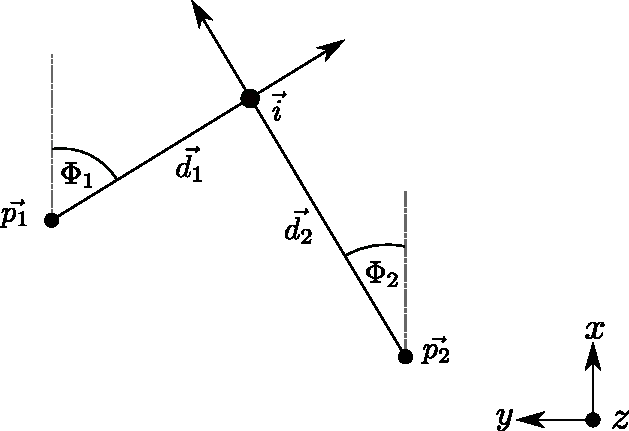
\includegraphics[width=0.50\textwidth]{figures/rays}
    \caption[Nomenclature for multi-agent localization algorithm]
            {Nomenclature for multi-agent localization algorithm.}
    \label{fig:03_rays}
\end{figure}
% -------------------------------------------------------------

% DEFINITION COVARIANCE MATRIX
The covariance matrix 
\bal
\frac{ix}{\delta \Phi_1} = \frac{(\cos(\Phi_2) \cdot (\cos(\Phi_1)^2 + \sin(\Phi_1)^2) \cdot ((p_{1y} - p_{2y}) \cdot \cos(\Phi_2) +
                                  (-p_{1x} + p_{2x}) \cdot \sin(\Phi_2)))}
                                  {(-\cos(\Phi_2) \cdot \sin(\Phi_1) + \cos(\Phi_1) \cdot \sin(\Phi_2))^2}
\eal


% -------------------------------------------------------------

% PSEUDO CODE UPDATING ALGORITHM
\begin{algorithm}[H]
    \caption{Bayesian Updating}\label{alg:03_multiAgentLoca}
    \begin{algorithmic}[1]
        \Procedure {WhistleLocalization}{$array<R>$}
            \For{$j \in 0:R.size()$}
                \For{$k \in j+1:R.size()$}
                    \State $\vec{i} \gets \Call{FindIntersection}{R[j], R[k]}$
                    \State $\textbf{\textit{C}} \gets \Call{CalulateCovariance}{R[j], R[k]}$
                    \If{first intersection found}
                        \State $\vec{\mu} \gets \vec{i}$
                        \State $\textbf{\textit{Q}} \gets \textbf{\textit{C}}$
                    \ElsIf{intersection found}
                        \State $\textbf{\textit{S}} \gets \textbf{\textit{Q}} + \textbf{\textit{C}}$
                        \State $\textbf{\textit{K}} \gets \textbf{\textit{Q}} \cdot \textbf{\textit{S}}^{-1}$
                        \State $\vec{\mu} \gets \vec{\mu} + \textbf{\textit{K}} \cdot (\vec{i} - \vec{\mu})$
                        \State $\textbf{\textit{Q}} \gets \textbf{\textit{Q}} - \textbf{\textit{K}} \cdot \textbf{\textit{Q}}$
                    \EndIf
                \EndFor
            \EndFor
            \State \textbf{return} $\vec{\mu}$
        \EndProcedure\vspace{12pt}
    \end{algorithmic}
\end{algorithm}
% -------------------------------------------------------------


For the evaluation of the methods, the team decision is implemented in
Python for offline analysis of the sample data additionally.

% Each value input is paired with the other rays. If they cross, the
% filter is updated with this intersection until all pairs of direction
% rays are being considered.
% \missing[]{More info}

% For the real case, a team whistle localization module is
% introduced into the HULKs' framework.
% Here, each robots fills the result of the determined direction into
% the team message.
% \missing[inline]{How this works.}

\subsection{Team Communication}
\label{subsec:03_teamCommunication}

To agree on a whistle position as multi-agent system, the detected sound source
direction is added into the team message as float.
Depending on the implementation, additional information like distance or
\ac{PSNR} can be appended.
